\vspace{-0.5em}
\section{Real-world deployment}
We deployed the proposed model into the SeoUHI system on the cloud to forecast the Urban Heat Island (UHI) effect. The system comprises four main modules. The data collector module continuously gathers real-time regional temperature data from the SDot project API. To address limited coverage and missing indoor temperature data, the data preprocessing module fills in gaps based on spatio-temporal neighbors. The prediction module forecasts regional temperatures for the next 24 hours at an hourly frequency, while the decision module identifies future hot times and locations, issuing UHI warnings. Additionally, the system automatically sends extreme heat warning emails to registered users during summer to protect vulnerable groups from heat exposure.

\begin{figure}[!b]
\centering
\vspace{-1em}
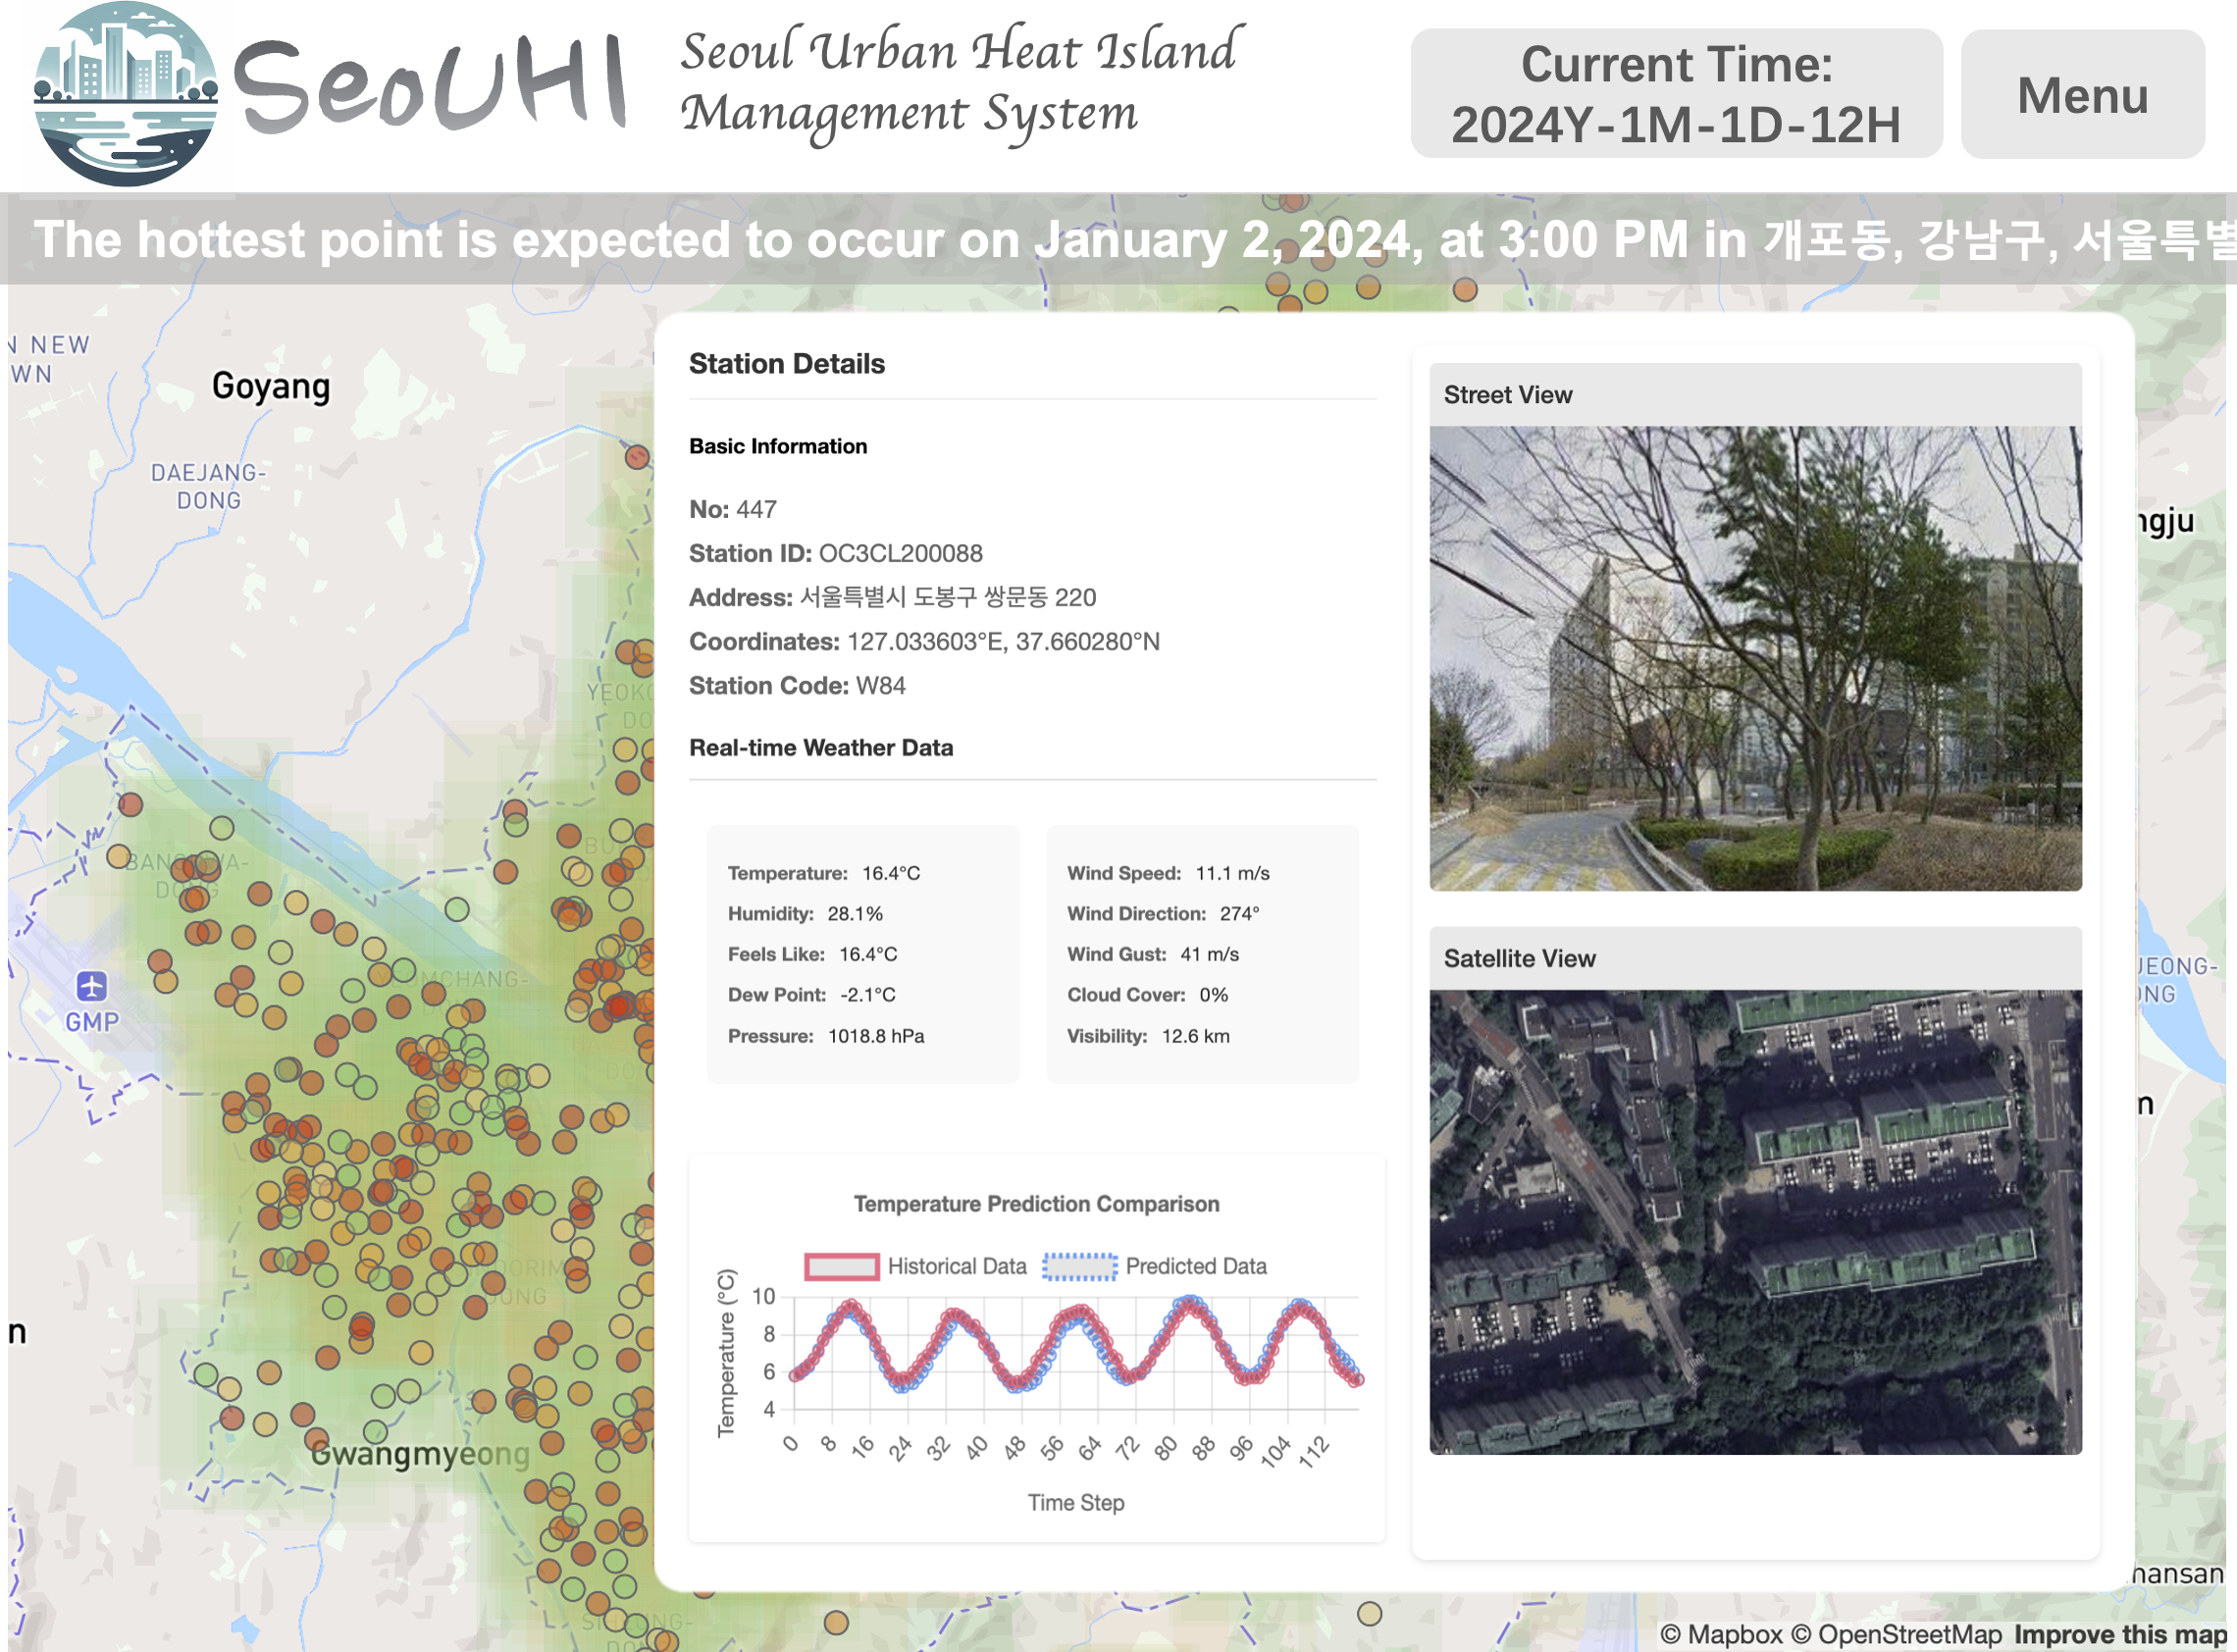
\includegraphics[width=1.0\linewidth]{resources/deploy.png}
\vspace{-2em}
\caption{Web platform of SeoUHI system}
\label{fig:depoly}
\end{figure}

The system features a user-friendly web interface, as shown in Figure \ref{fig:depoly}, displaying a dynamic heat map of Seoul. Users can select a target region to view predicted temperatures in a line graph format, allowing for comparisons between predicted and actual temperatures over different time spans. The predictive system executes hourly updates for the 947 temperature stations in Seoul. To maintain accuracy, the core model is retrained monthly with the latest regional temperature data, benefiting from its lightweight architecture. Our data-driven model does not rely on physical rule-based simulation, eliminating the need for detailed physical information or extensive computational resources, which facilitates practical deployment. However, it requires hourly average regional temperature data, necessitating the installation of temperature sensors within the city, currently limiting deployment to the Seoul area.